\chapter{Experiments}

In this chapter \ldots 

\section{Quantitative Quality Measures}
\label{sec:measures}
\textcolor{red}{THIS SECTION COULD ALSO BE IN THE METHODS CHAPTER}

example equation
\begin{align}
    MSE(a,b) &= \frac{1}{N}\sum_{n=1}^N||a_n-b_n||_2^2
    \label{eq:mse}
\end{align}
% % features, model, evaluation


\section{Classification X}
\textcolor{red}{EXAMPLES FOR REFERENCES AND CITATION OF CODE: ADD ENTRIES TO references.bib} 
The model described in Sec.~\ref{sec:model_age}... 

implementation is based on \cite{vgg_github_2020}, which was combined with \cite{lia_corrales_2015_15991}. 

measure for evaluation Sec.~\ref{sec:measures}, MSE \eqref{eq:mse}

\section{Group Analysis}

In Fig.~\ref{fig:subfigs} it can be seen \ldots 
Fig.~\ref{fig:subfigs}\subref{subfig:input} the original image, \ldots Fig.~\ref{fig:subfigs}\subref{subfig:detect} \ldots 

\begin{figure}[htb] % "H"ere, "T"op "B"ottom
    \centering
    \subfloat[original]{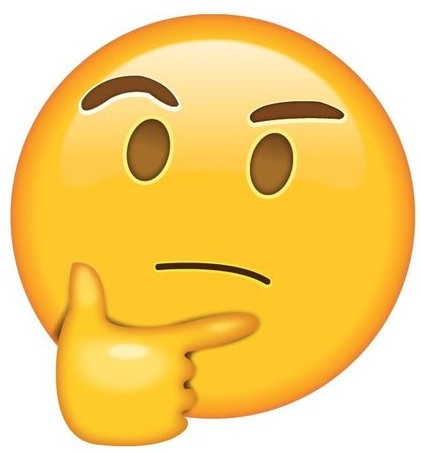
\includegraphics[width=0.3\textwidth]{figs/dummy_img} \label{subfig:input}}
    \subfloat[detected]{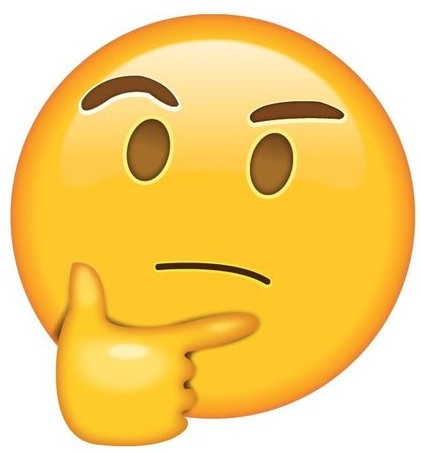
\includegraphics[width=0.25\textwidth]{figs/dummy_img} \label{subfig:detect}}
    \\ % new line if needed
    \subfloat[example 2]{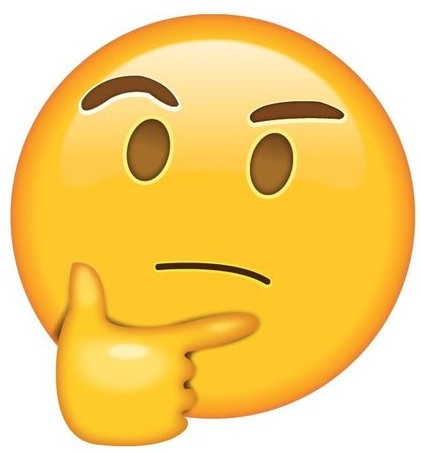
\includegraphics[width=0.48\textwidth]{figs/dummy_img}}
    \subfloat[estimated]{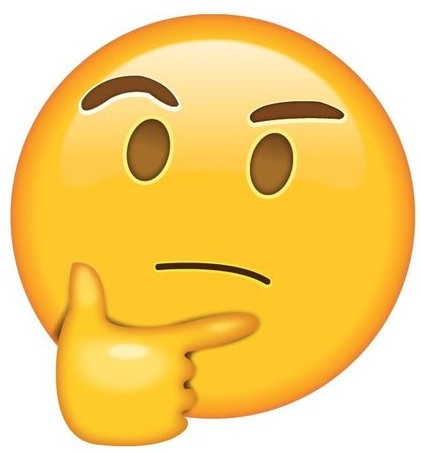
\includegraphics[width=0.48\textwidth]{figs/dummy_img} \label{subfig:ex2}}
    \caption{%
    There should be a short description here. More details in the text: \protect\subref{subfig:input} original image, \protect\subref{subfig:detect} 
    \textcolor{red}{2DO: adapt content, size and description. You can put it all in one row, too.}
    }
    \label{fig:subfigs}
\end{figure}



